\subsection{Booster Synchrotron}

Η δέσμη των βαρέων ίοντων, εξέρχεται από το σύστημα EBIS-RFQ-HI Linac όχι σε συνεχή μορφή αλλά παλμικά, και οδηγείται στον επόμενο προεπιταχυντή, τον Booster Synchrotron (Εικόνα (\ref{fig2.5})) μέσω του Beam Port. Για τον RHIC εισέρχονται στον Booster Synchrotron $^3He^{2+}, ^4He^{1+}, ^4He^{2+}$, $ Cu^{11+}, Au^{32+}, U^{39}$ με ενέργεια έως 2MeV/n. 

	\begin{figure}[h!]
		\centering
		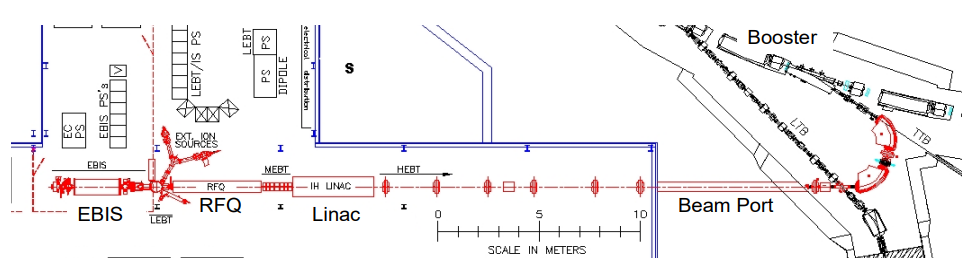
\includegraphics[scale=0.5]{Accelerating_System/1st_stage.png}
		\caption{1ο στάδιο επιτάχυνσης}
		\label{fig2.5}
	\end{figure}
	
	Πριν την ολοκλήρωση της κατασκευής του το 1990, όταν ακόμη ο κύριος επιταχυντής ήταν ο AGS και όχι ο RHIC,\footnote{Πλέον o AGS λειτουργεί ως προεπιταχυντής για τον RHIC} δεν ήταν δυνατή η επιτάχυνση όλων των ιόντων στον AGS. 
	Επειδή ο AGS μπορεί να επιταχύνει σχεδόν πλήρως ιονισμένα άτομα, θα έπρεπε να τα έχουμε ιονίσει πρωτού τα εισάγουμε σε αυτόν, επομένως
	%και ο εν λόγω ιονισμός στο πρόγραμμα βαρέων ιόντων του AGS εκείνης της εποχής ήταν αδύνατος για άτομα βαρύτερα του Θείου.
	ο ρόλος του Booster Synchrotron είναι να προεπιταχύνει τα ιόντα και ταυτόχρονα να τα ιονίσει περεταίρω ώστε να μπορούν να επιταχυνθούν επιτυχώς στον AGS. Πέρα από τα ιόντα, έχει σημαντικό ρόλο και στην προεπιτάχυνση των πρωτονίων όπως θα δούμε στην συνέχεια.
	
	Έχει περιφέρεια 207.78m, το 1/4 της περιφέρειας του AGS και όντας σύγχροτρο αποτελείται από ένα πλέγμα κυψελίδων εντός των οποίων η ταχύτητα της δέσμης αλλάζει κατεύθυνση και μέτρο.
	 Τα κελιά που έχουν χρησιμοποιηθεί είναι τύπου FODO (\textbf{F}ocusing - Χώρος Ολίσθησης \textbf{O} - \textbf{D}efocusing - \textbf{O}), αποτελούνται δηλαδή από δύο τετραπολικούς μαγνήτες με αντίθετες πολικότητες οι οποίοι εστιάζουν την δέσμη σε διαφορετικές κατευθύνσεις. Ενδιάμεσα από αυτούς τους μαγνήτες καθώς και στο τέλος της κεψελίδας υπάρχει ένα διπολικός μαγνήτης ο οποίος χρησιμεύει για να στρίψει την δέσμη. Στον συγκεκριμένο επιταχυντή λείπει ο πρώτος διπολικός από κάθε δεύτερο κελί.
	 Συνολικά έχει 6 συστοιχείες εκ των οποίων η κάθε μία 4 FODO κυψιλίδες 
	Η μέγιστη ενέργεια με την οποία εξάγονται τα βαρέα ιόνται από τον Booster Synchrotron ποικίλλει από 0.35-1GeV ανάλογα το ιόν